\chapter{具体需求}
下面详细描述具体的需求。

\section{功能需求}

%本子章节应描述软件产品的输入怎样被转换成输出。它描述了软件必须执行的基本动作。 

%对每一类功能或有时对每一个单独的功能,必须描述输入、处理、输出方面的需求。这些通常以下面四个子段落来组织:
\subsection{开发者端.应用管理}
需求编码为SRS\_Dev\_App\_P01

\subsubsection{介绍}
本小节主要介绍了开发者进行应用管理的需求,包括应用的上传、更新、删除等等。

需求编码为SRS\_Dev\_App\_P01\_F01

\subsubsection{输入}

需求编码为SRS\_Dev\_App\_P01\_I01

针对开发者对其应用的管理需求,其输入数据应当是某个应用和对该应用的操作,数据来源均为开发者,具体如下:

\begin{longtable}[]{@{}ll@{}}
\toprule
数据名称 & 数据要求\tabularnewline
\midrule
\endhead
对应用的操作 & 上传、更新、删除之一\tabularnewline
应用id & 应用id为该开发者开发的应用之一(更新、删除),应用id首次出现(应用上传)\tabularnewline
应用 & 合法的应用程序 \tabularnewline
\bottomrule
\end{longtable}

\subsubsection{处理}
对输入进行处理,得到输出内容,需求编码为SRS\_Dev\_App\_P01\_H01

\textbf{A. 输入数据的有效性检测}

\begin{longtable}[]{@{}ll@{}}
\caption{开发者端进行应用管理输入数据的有效性检测}\label{tab:developer_app_management}\\
\toprule
数据名称 & 数据要求\tabularnewline
\midrule
\endhead
对应用的操作 & 上传、更新、删除之一\tabularnewline
应用id & 应用id为该开发者开发的应用之一(更新、删除),应用id首次出现(应用上传)\tabularnewline
应用 & 合法的应用程序 \tabularnewline
\bottomrule
\end{longtable}

见表\ref{tab:developer_app_management}

\textbf{B. 操作的确切次序,包括各事件的时序}

\begin{figure}[ht]
	\centering
	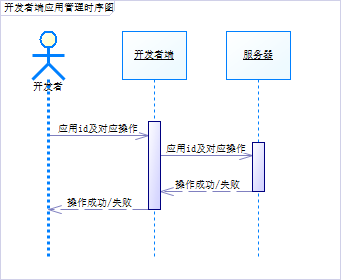
\includegraphics[width=14cm]{developer_app_order.png}
	\caption{开发者端进行应用管理的事件时序} \label{fig:developer_app_order}
\end{figure}
见图\ref{fig:developer_app_order}

\textbf{C. 对异常情况的回应}

\begin{longtable}{|c|p{6cm}|p{6cm}|}
\caption{开发者管理系统异常处理}\label{tab:developer_app_management_exception}\\
\hline
\textbf{异常类型} & \textbf{异常描述} & \textbf{异常处理}\\
\hline
\endfirsthead

\hline
\textbf{异常类型} & \textbf{异常描述} & \textbf{异常处理}\\
\hline
\endhead
\hline 
\endfoot
\hline
\endlastfoot
服务器异常 & 
与服务器采用网络通信,限定时间内没有收到应答 &
储存错误状态,提示开发者检查网络连接\\
应用id不合法 
& 删除或更新应用时,id对应的应用并不存在开发者所开发的应用中
& 提示开发者重新操作\\
应用不合法
& 上传的不是合法的应用程序
&提示开发者重新操作\\
\end{longtable}

表\ref{tab:developer_app_management_exception}概要性描述了几个可能出现的错误,以及相关的解决方案。
更加详细的方案见概要设计。

\textbf{D. 用于把系统输入转换到相应输出的任何方法}
只需要将服务器返回的结果返回给开发者即可,不需要额外的数学算法或操作逻辑等等。
		
\textbf{E. 对输出数据的有效性检测}

此处只考虑开发者端返回e给开发者的数据,返回给服务器的数据参见服务器端.应用管理系统。
输出数据为:操作的成功与否以及可能的错误信息,具体如下:
\begin{longtable}{|p{7cm}|p{7cm}|}
\caption{开发者端应用管理输出有效性检测}\label{tab:concrete_dev_sys_output_valid} \\
\hline
\textbf{输出内容} & \textbf{有效性检测} \\
\hline
\endfirsthead
\hline
\textbf{输出内容} & \textbf{有效性检测} \\
\hline
\endhead
\hline 
\endfoot
\hline
\endlastfoot

操作结果 & 布尔量,成功或失败 \\
错误信息 & 操作成功则为空,操作失败则为一个字符串,建议开发者下一步的操作,长度暂定为128byte\\
\end{longtable}


\subsubsection{输出}
需求编码为SRS\_Dev\_App\_P01\_O01

参见上一节E对输出数据的有效性检测。

\subsection{开发者端.信息反馈}
本小节主要描述了开发者获取信息反馈的需求,比如查询应用评价等等。

需求编码为SRS\_Dev\_Info\_P01

\subsubsection{介绍}
逐条列出与本特性相关的功能需求。包括项目如何响应预期的错误输入,非法条件和无效输入。需求应该简明,完整,不含糊,可验证,必要的。 当需要的信息不确定的时候使用“待定”。
需求编码为SRS\_Dev\_Info\_P01\_F01

\subsubsection{输入}

需求编码为SRS\_Dev\_Info\_P01\_I01
针对开发者获取关于其应用的信息的需求,输入数据应当包括:应用id、具体的查询管理需求等等,数据来源均为开发者(此处不考虑隐式的数据来源,即服务器),具体如下:

\begin{longtable}[]{@{}ll@{}}
\toprule
数据名称 & 数据要求\tabularnewline
\midrule
\endhead
应用id & 应用id为该开发者开发的应用之一\tabularnewline
具体需求 & 应用信息查询、评论回复、收入查询、收入提现、收入转账等命令之一\tabularnewline
评论回复 & 当且仅当具体需求是评论回复时不为空,为一个字符串,长度暂定为256字节\tabularnewline
银行账号 & 当且仅当具体需求是收入提现或转账时不为空,为一个合法的银行账号\tabularnewline
\bottomrule
\end{longtable}

\subsubsection{处理}
对输入进行处理,得到输出内容,
需求编码为SRS\_Dev\_Info\_P01\_H01

\textbf{A. 输入数据的有效性检测}

\begin{longtable}[]{@{}ll@{}}
\caption{开发者端信息反馈的输入数据的有效性检测}\label{tab:developer_app_info}\\
\toprule
数据名称 & 数据要求\tabularnewline
\midrule
\endhead
具体需求 & 应用信息查询、评论回复、收入查询、收入提现、收入转账等命令之一\tabularnewline
应用id & 当且仅当具体需求是应用信息查询时不为空,应用id为该开发者开发的应用之一\tabularnewline
评论回复 & 当且仅当具体需求是评论回复时不为空,为一个字符串,长度暂定为256字节\tabularnewline
银行账号 & 当且仅当具体需求是收入提现或转账时不为空,为一个合法的银行账号\tabularnewline
\bottomrule
\end{longtable}

见表\ref{tab:developer_app_info}

\textbf{B. 操作的确切次序,包括各事件的时序}

\begin{figure}[ht]
	\centering
	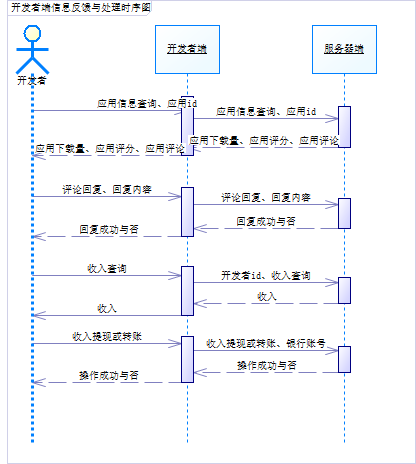
\includegraphics[width=14cm]{developer_info_order.png}
	\caption{开发者获取信息反馈并处理的事件时序} \label{fig:developer_info_order}
\end{figure}
见图\ref{fig:developer_info_order}

\textbf{C. 对异常情况的回应}

\begin{longtable}{|c|p{6cm}|p{6cm}|}
\caption{开发者端信息反馈异常处理}\label{tab:developer_info_exception}\\
\hline
\textbf{异常类型} & \textbf{异常描述} & \textbf{异常处理}\\
\hline
\endfirsthead

\hline
\textbf{异常类型} & \textbf{异常描述} & \textbf{异常处理}\\
\hline
\endhead
\hline 
\endfoot
\hline
\endlastfoot
服务器异常 & 
与服务器采用网络通信,限定时间内没有收到应答 &
储存错误状态,提示开发者检查网络连接\\
应用id不合法 
& id对应的应用并不存在开发者所开发的应用中
& 提示开发者重新操作\\
银行账号不存在
& 用于提现或转账的银行账号不存在
&提示开发者提供正确的银行账号\\
转账或提现金额过大
& 转账或提现金额超过限额
& 提示开发者减小提现或转账金额
\end{longtable}

表\ref{tab:developer_info_exception}概要性描述了几个可能出现的错误,以及相关的解决方案。
更加详细的方案见概要设计。

\textbf{D. 用于把系统输入转换到相应输出的任何方法}
只需要将服务器返回的结果返回给开发者即可,不需要额外的数学算法或操作逻辑等等。
		
\textbf{E. 对输出数据的有效性检测}

此处只考虑开发者端返回给开发者的数据,返回给服务器的数据参见服务器端.应用管理系统。具体如下:
\begin{longtable}{|p{7cm}|p{7cm}|}
\caption{开发者端信息反馈输出有效性检测}\label{tab:concrete_dev_sys_output_valid} \\
\hline
\textbf{输出内容} & \textbf{有效性检测} \\
\hline
\endfirsthead
\hline
\textbf{输出内容} & \textbf{有效性检测} \\
\hline
\endhead
\hline 
\endfoot
\hline
\endlastfoot

下载量 & 整型数据,非负整数 \\
评论 & 字符串\\
收入 & 浮点型数据,非负数\\
操作结果 & 布尔量

\end{longtable}


\subsubsection{输出}
需求编码为SRS\_Dev\_Info\_P01\_O01

参见上一节E对输出数据的有效性检测。


{\color{red}
\subsection{开发者端.应用开发界面}

需求编码为SRS\_Dev\_Dev\_P01
\subsubsection{介绍}
此处提供开发的界面,实现开发-上线一体化,整个应用商店实现完整的生态链。 

为了便于开发,以及免去开发者的下载,
本系统也提供基于浏览器的开发系统。只需与服务器交换数据,就可以使用本系统提供的
编译运行环境。

需求编码为SRS\_Dev\_Dev\_P01\_F01
\subsubsection{输入}

本支系统针对开发者端,数据来源都是开发者端的应用。

需求编码为SRS\_Dev\_Dev\_P01\_I01

输入数据要求

\begin{longtable}[]{@{}ll@{}}
\toprule
数据名称 & 数据要求\tabularnewline
\midrule
\endhead
指令 & 开发界面按键\tabularnewline
code & 通过语法检查  \tabularnewline
\bottomrule
\end{longtable}

\subsubsection{处理}

对输入进行处理,得到输出内容

需求编码为SRS\_Dev\_Dev\_P01\_H01

\textbf{A. 输入数据的有效性检测}

\begin{longtable}[]{@{}ll@{}}
\caption{开发界面输入的有效性检测}\label{tab:dev_dev_input_valid}\\
\toprule
数据名称 & 数据要求\tabularnewline
\midrule
\endhead
指令 & 界面的按键或者命令行并通过简单的语法检查\tabularnewline
code & 通过相应编程语言的语法检查  \tabularnewline
\bottomrule
\end{longtable}

见表\ref{tab:dev_dev_input_valid}

\textbf{B. 操作的确切次序,包括各事件的时序}

由于是在线开发,开发者界面会传输到服务器进行数据的处理,所以其处理的时序也就是先进行简单的语法检查,如果出错,
就直接报错,否则传输到服务器高性能计算中心进行编译运行处理。

\textbf{C. 对异常情况的回应}

\begin{longtable}{|c|p{6cm}|p{6cm}|}
\caption{开发界面异常处理}\label{tab:dev_dev_exception} \\
\hline
\textbf{异常类型} & \textbf{异常描述} & \textbf{异常处理}\\
\hline
\endfirsthead
%\multicolumn{3}{c}{\tablename\ \thetable\ -- \textit{Continued from previous page}} \\
\hline
\textbf{异常类型} & \textbf{异常描述} & \textbf{异常处理}\\
\hline
\endhead
\hline 
%\multicolumn{3}{r}{\textit{Continued on next page}} \\
\endfoot
\hline
\endlastfoot
通信失败 & 
与服务器采用网络通信,限定时间内没有收到应答或者没有新的请求 &
储存错误状态,储存编辑到本地,断开连接\\
语法错误 & 对代码或者命令进行本地语法检查的时候发现语法错误 & 
直接显示出错误信息,并暂停数据传输给服务器\\
攻击检测 & 网络安全相关,比如检测到某个账户持续性注册注销 &
停止对该帐号的应答,并且设定恢复时间\\
\end{longtable}

表\ref{tab:dev_dev_exception}概要性描述了几个可能出现的错误,以及相关的解决方案。
更加详细的方案见概要设计。



\textbf{D. 用于把系统输入转换到相应输出的任何方法}

输入转化成输出,需要经过两个阶段,一是进行语法检查,如果检查出错误,就显示错误信息,
否则传输给服务器编译运行,在返回浏览器数据,并显示。

\textbf{E. 对输出数据的有效性检测}

返回数据无需检查,因为从服务器传输过来的数据为字符或者实时界面数据,可以直接在浏览器上显示。

\subsubsection{输出}

需求编码为SRS\_Dev\_Dev\_P01\_O01

输出数据也就是字符型的信息与界面数据

}




\subsection{服务器端.开发者管理系统}
需求编码为SRS\_Server\_Dev\_P01
\subsubsection{介绍}
集中对开发者的活动进行管理。包括注册与注销,个人基本信息维护,开发的应用列表。
需求编码为SRS\_Server\_Dev\_P01\_F01
\subsubsection{输入}

本支系统针对开发者端,数据来源都是开发者端的应用

需求编码为SRS\_Server\_Dev\_P01\_I01

输入数据要求

\begin{longtable}[]{@{}ll@{}}
\toprule
数据名称 & 数据要求\tabularnewline
\midrule
\endhead
用户名 & 可以接收验证码的邮箱\tabularnewline
密码 &
至少8个字符;必须包含大写与小写字母;至少一个数字;\tabularnewline
\bottomrule
\end{longtable}

输入数据根据不同功能需求的开发者端口要求

\begin{longtable}[]{@{}lll@{}}
\toprule
开发者端功能需求 & 用户名 & 密码\tabularnewline
\midrule
\endhead
注册 & YES & NO\tabularnewline
登录 & YES & YES\tabularnewline
注销 & YES & YES\tabularnewline
找回密码 & YES & NO\tabularnewline
\bottomrule
\end{longtable}

\subsubsection{处理}

对输入进行处理,得到输出内容

需求编码为SRS\_Server\_Dev\_P01\_H01

\textbf{A. 输入数据的有效性检测}

\begin{longtable}[]{@{}ll@{}}
\caption{开发者系统输入的有效性检测}\label{tab:developer_sys_input_valid}\\
\toprule
数据名称 & 数据要求\tabularnewline
\midrule
\endhead
用户名 & 含有@的正常邮箱,是否能接收验证码在此处的初始检测不作要求\tabularnewline
密码 &
至少8个字符;必须包含大写与小写字母;至少一个数字;\tabularnewline
\bottomrule
\end{longtable}

见表\ref{tab:developer_sys_input_valid}

\textbf{B. 操作的确切次序,包括各事件的时序}

\begin{figure}[ht]
	\centering
	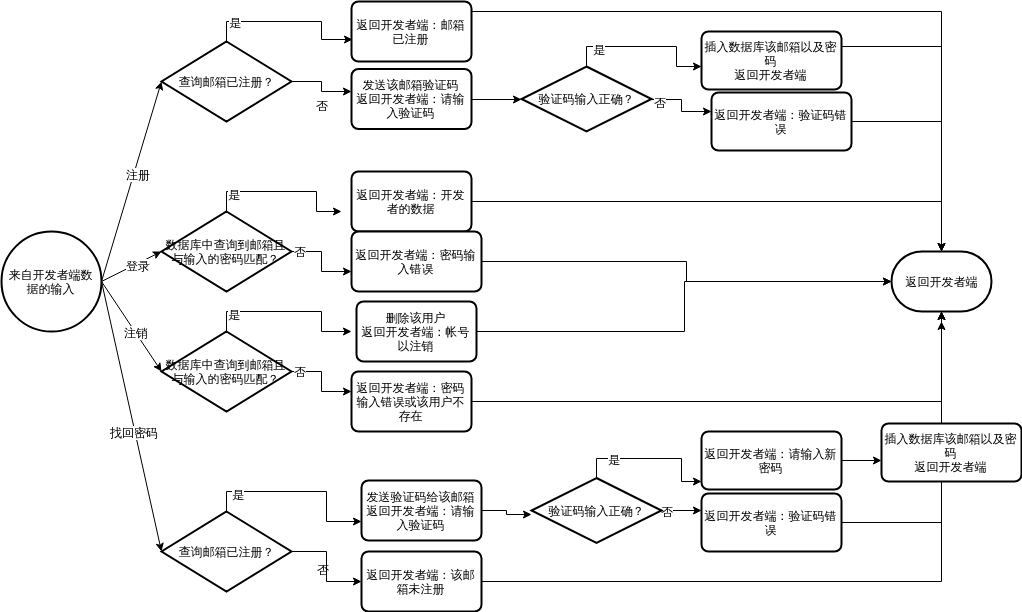
\includegraphics[width=14cm]{concrete_dev_sys.png}
	\caption{开发者管理系统事件时序} \label{fig:concrete_developer}
\end{figure}


数据流图\ref{fig:concrete_developer}明确表示了开发者管理系统的运行


\textbf{C. 对异常情况的回应}

\begin{longtable}{|c|p{6cm}|p{6cm}|}
\caption{开发者管理系统异常处理}\label{tab:developer_exception} \\
\hline
\textbf{异常类型} & \textbf{异常描述} & \textbf{异常处理}\\
\hline
\endfirsthead
%\multicolumn{3}{c}{\tablename\ \thetable\ -- \textit{Continued from previous page}} \\
\hline
\textbf{异常类型} & \textbf{异常描述} & \textbf{异常处理}\\
\hline
\endhead
\hline 
%\multicolumn{3}{r}{\textit{Continued on next page}} \\
\endfoot
\hline
\endlastfoot
通信失败 & 
与开发者端采用网络通信,限定时间内没有收到应答或者没有新的请求 &
储存错误状态,断开连接\\
数据库异常 & 数据库出现异常,比如数据库断联,数据库储存满 &
暂停服务,通知管理员\\
攻击检测 & 网络安全相关,比如检测到某个账户持续性注册注销 &
停止对该帐号的应答,并且设定恢复时间\\
\end{longtable}

表\ref{tab:developer_exception}概要性描述了几个可能出现的错误,以及相关的解决方案。
更加详细的方案见概要设计。



\textbf{D. 用于把系统输入转换到相应输出的任何方法}

开发者系统的处理主要是对数据库的访问处理,根据数据流图\ref{fig:concrete_developer}的
业务逻辑处理即可,并不需要额外的方程式或者数学算法。
		
\textbf{E. 对输出数据的有效性检测}

输出内容分为两类,一是返回给开发者端的提示与错误信息:主体为文本内容,并且为每个信息配有unsigned int类型的描述符。
相关信息有:邮箱已注册;邮箱未注册;输入验证码;密码错误;

\begin{longtable}{|p{7cm}|p{7cm}|}
\caption{开发者管理系统输出有效性检测}\label{tab:concrete_dev_sys_output_valid} \\
\hline
\textbf{输出内容} & \textbf{有效性检测} \\
\hline
\endfirsthead
%\multicolumn{2}{c}{\tablename\ \thetable\ -- \textit{Continued from previous page}} \\
\hline
\textbf{输出内容} & \textbf{有效性检测} \\
\hline
\endhead
\hline 
%\multicolumn{2}{r}{\textit{Continued on next page}} \\
\endfoot
\hline
\endlastfoot

用户名 & 不为空,默认为邮箱,可进行修改 \\
姓名 & 不为空,中文或英文字符串,Unicode格式,限制长度64bytes \\
性别 & 可为空,男/女 \\
年龄 & 可为空,类型为unsigned int \\
开发的应用ID & 可为空,类型为unsigned int, 全局唯一code \\
收入查询 & 不可为空,类型为unsigned int, 如果没有收益则为0 \\
收入提现 & 可为空,提现码,需要与银行账户、支付宝、微信等接入 \\
应用评分与评价 & 可为空,返回一个表格,主码为应用ID, 评分为0~5区间的float类型,评价为字符串序列 \\

\end{longtable}


另外就是返回开发者的信息,
见表\ref{tab:concrete_dev_sys_output_valid}

\subsubsection{输出}

需求编码为SRS\_Server\_Dev\_P01\_O01

\begin{longtable}{|p{3cm}|p{4cm}|p{1cm}|p{6cm}|}
\caption{开发者管理系统输出}\label{tab:concrete_dev_sys_output} \\
\hline
\textbf{输出内容} & \textbf{输出位置} & \textbf{数量}  & \textbf{非法值处理错误信息}    \\
\hline
\endfirsthead
%\multicolumn{4}{c}{\tablename\ \thetable\ -- \textit{Continued from previous page}} \\
\hline
\textbf{输出内容} & \textbf{输出位置} & \textbf{数量}  & \textbf{非法值处理错误信息}  \\
\hline
\endhead
\hline 
%\multicolumn{4}{r}{\textit{Continued on next page}} \\
\endfoot
\hline
\endlastfoot

用户名 & 开发者端 & 1 & 用户名不存在\\
姓名 & 开发者端 & 1 & 姓名字符含有非法字符\\
性别 & 开发者端 & 0/1 & 无\\
年龄 & 开发者端 & 0/1 & 无\\
开发的应用ID & 开发者端 & $\ge 0$ & 无\\
收入查询 & 开发者端 & 1 & 无\\
收入提现 & 开发者端 & 0/1 & 无\\
应用评分与评价 & 开发者端 & $\ge 0$ & 无\\
注册的用户名密码 & 数据库 & 1 & 该用户已注册\\
注销的用户名密码 & 数据库 & 1 & 该用户未注册 \\

\end{longtable}
	
对输出数据的管理见表\ref{tab:concrete_dev_sys_output}




\subsection{服务器端.应用管理系统}
需求编码为SRS\_Server\_App\_P01

\subsubsection{介绍}
集中对应用数据的的管理,包括两大方面,一是应用信息的维护与更新,二是应用本身的上传、更新、下载、删除管理。

需求编码为SRS\_Server\_App\_P01\_F01

\subsubsection{输入}

需求编码为SRS\_Server\_App\_P01\_I01

\begin{longtable}{|p{3cm}|p{4cm}|p{1cm}|p{6cm}|}
\caption{应用管理系统输入}\label{tab:concrete_app_sys_input} \\
\hline
\textbf{输入内容} & \textbf{输入来源} & \textbf{数量}  & \textbf{有效范围}    \\
\hline
\endfirsthead
%\multicolumn{4}{c}{\tablename\ \thetable\ -- \textit{Continued from previous page}} \\
\hline
\textbf{输入内容} & \textbf{输入来源} & \textbf{数量}  & \textbf{有效范围}  \\
\hline
\endhead
\hline 
%\multicolumn{4}{r}{\textit{Continued on next page}} \\
\endfoot
\hline
\endlastfoot

开发者登录并提取应用信息 & 开发者端 & 1 & 系统内部定义开发者登录成功的描述符 \\
开发者登录并上传应用 & 开发者端 & 1 & 应用的合法性 \\
开发者登录并更新应用 & 开发者端 & 1 & 应用的合法性 \\
开发者登录并删除应用 & 开发者端 & 1 & 应用属于该开发者 \\
用户登录并搜索应用名 & 用户端 & 1 & 系统内部定义用户登录成功的描述符 \\
用户登录并查看购买的应用 & 用户端 & 1 & 系统内部定义用户登录成功的描述符 \\
游客搜索应用名 & 用户端 & 1 & 任何字符 \\
游客查看应用的下载量/评分/评价 & 用户端 &1 & 该应用存在 \\

\end{longtable}


对输入的管理信息见表\ref{tab:concrete_app_sys_input}	

\subsubsection{处理}
包含对输入数据所执行的所有操作和如何获得输出的过程

需求编码为SRS\_Server\_App\_P01\_H01

\textbf{A. 输入数据的有效性检测}

\begin{longtable}{|p{3cm}|p{11cm}|}
\caption{应用管理系统输入有效性检测}\label{tab:concrete_app_sys_input_valid} \\
\hline
\textbf{输入内容} & \textbf{有效性检测}    \\
\hline
\endfirsthead
%\multicolumn{2}{c}{\tablename\ \thetable\ -- \textit{Continued from previous page}} \\
\hline
\textbf{输入内容} & \textbf{有效性检测}   \\
\hline
\endhead
\hline 
%\multicolumn{2}{r}{\textit{Continued on next page}} \\
\endfoot
\hline
\endlastfoot
开发者登录 & 符合登录描述符规范 \\
用户登录 & 符合登录描述符规范 \\
应用名搜索 & 任何字符 \\
应用上载 & 符合应用程序规范的应用,后期需要接受应用审查 \\
评分 & 0-5 unsigned int \\
评价 & 字符串,unicode,128 bytes \\
\end{longtable}
	
输入数据的有效性检测见表\ref{tab:concrete_app_sys_input_valid}


\textbf{B. 操作的确切次序,包括各事件的时序}

\begin{figure}[ht]
	\centering
	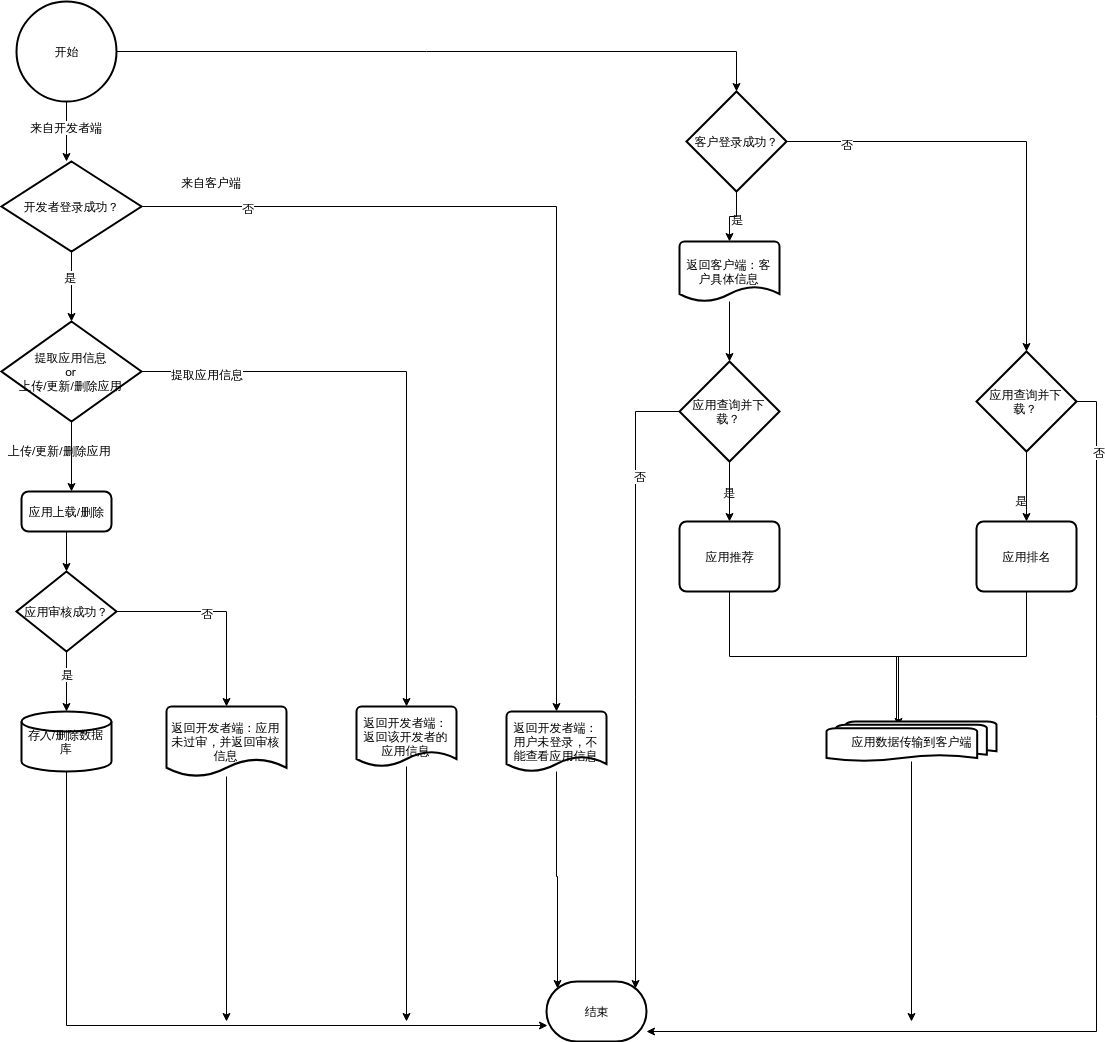
\includegraphics[width=14cm]{concrete_app_sys.png}
	\caption{应用管理系统事件时序} \label{fig:concrete_app_sys}
\end{figure}

对应用管理系统的事件时序见图\ref{fig:concrete_app_sys}

\textbf{C. 对异常情况的回应}

\begin{longtable}{|p{3cm}|p{5cm}|p{6cm}|}
\caption{应用管理系统异常处理}\label{tab:concrete_app_sys_exception} \\
\hline
\textbf{异常类型} & \textbf{异常描述} & \textbf{异常处理}\\
\hline
\endfirsthead
%\multicolumn{3}{c}{\tablename\ \thetable\ -- \textit{Continued from previous page}} \\
\hline
\textbf{异常类型} & \textbf{异常描述} & \textbf{异常处理}\\
\hline
\endhead
\hline 
%\multicolumn{3}{r}{\textit{Continued on next page}} \\
\endfoot
\hline
\endlastfoot
通信失败 & 
与开发者或用户端端采用网络通信,限定时间内没有收到应答或者没有新的请求 &
储存错误状态,断开连接\\
数据库异常 & 数据库出现异常,比如数据库断联,数据库储存满 &
暂停服务,通知管理员\\
攻击检测 & 网络安全相关,比如检测到某个账户持续性刷评 &
停止对该帐号的应答,并且设定恢复时间\\
\end{longtable}

表\ref{tab:concrete_app_sys_exception}概要性描述了几个可能出现的错误,以及相关的解决方案。
更加详细的方案见概要设计。


\textbf{D. 用于把系统输入转换到相应输出的任何方法}

\begin{longtable}{|p{3cm}|p{11cm}|}
\caption{应用管理系统转换处理}\label{tab:concrete_app_sys_transform} \\
\hline
\textbf{过程名} & \textbf{处理方式} \\
\hline
\endfirsthead
%\multicolumn{2}{r}{\tablename\ \thetable\ -- \textit{Continued from previous page}} \\
\hline
\textbf{过程名} & \textbf{处理方式}\\
\hline
\endhead
\hline 
%\multicolumn{2}{r}{\textit{Continued on next page}} \\
\endfoot
\hline
\endlastfoot
应用审核 & 采用AI审核与人工审核结合的办法。 AI审核包括试运行、关键词检测、内容分析、抄袭检测、评分估计等方式;
人工审核指AI审核后不通过返回给开发者,并且开发者提出异议的时候人工检测\\
应用排名 & 针对未登录的游客,主体按照用户评分推荐,给新出的应用分流,给持续增加使用人数与评分的应用更多流量 \\
应用推荐 & 针对已经登录的用户,除了使用应用排名给出的应用推荐,还要结合用户的使用习惯以及同龄人的喜好给予推荐 \\

\end{longtable}
		
\textbf{E.	对输出数据的有效性检测}

\begin{longtable}{|p{3cm}|p{11cm}|}
\caption{应用管理系统输出有效性检测}\label{tab:concrete_app_sys_output_valid} \\
\hline
\textbf{输出内容} & \textbf{有效性检测}    \\
\hline
\endfirsthead
%\multicolumn{2}{c}{\tablename\ \thetable\ -- \textit{Continued from previous page}} \\
\hline
\textbf{输出内容} & \textbf{有效性检测}   \\
\hline
\endhead
\hline 
%\multicolumn{2}{r}{\textit{Continued on next page}} \\
\endfoot
\hline
\endlastfoot
应用下载数据 & MD5检验未损坏 \\
搜索获得的应用列表 & 包含应用名、应用ID、应用图片、应用简介、应用评分与评价\\
开发者的应用列表 & 除了上述内容外,还包含应用的更新记录、下载量分析、评分分析、评价分类汇总\\
\end{longtable}
对输出的有效性检测见表\ref{tab:concrete_app_sys_output_valid}


\subsubsection{输出}

需求编码为SRS\_Server\_App\_P01\_O01

\begin{longtable}{|p{3cm}|p{4cm}|p{1cm}|p{6cm}|}
\caption{应用管理系统输出}\label{tab:concrete_app_sys_output} \\
\hline
\textbf{输出内容} & \textbf{输出位置} & \textbf{数量}  & \textbf{非法值处理错误信息}    \\
\hline
\endfirsthead
%\multicolumn{4}{c}{\tablename\ \thetable\ -- \textit{Continued from previous page}} \\
\hline
\textbf{输出内容} & \textbf{输出位置} & \textbf{数量}  & \textbf{非法值处理错误信息}  \\
\hline
\endhead
\hline 
%\multicolumn{4}{r}{\textit{Continued on next page}} \\
\endfoot
\hline
\endlastfoot
应用下载数据 & 用户端 & 1 & 重新传输数据\\
搜索获得的应用列表 & 用户端 & $\ge 0$ & 不存在时返回0\\
开发者的应用列表 & 用户端 & $\ge 0$ & 不存在时返回0\\
\end{longtable}
	
对输出数据的管理见表\ref{tab:concrete_app_sys_output}


\subsection{服务器端.用户管理系统}
需求编码为SRS\_Server\_User\_P01
\subsubsection{介绍}
集中对用户的活动进行管理。包括注册与注销,个人基本信息维护,下载/购买的应用列表。

需求编码为SRS\_Server\_App\_P01\_F01
\subsubsection{输入}

需求编码为SRS\_Server\_App\_P01\_I01

本支系统针对用户端,数据来源都是用户端的应用

输入数据要求

\begin{longtable}[]{@{}ll@{}}
\toprule
数据名称 & 数据要求\tabularnewline
\midrule
\endhead
用户名 & 可以接收验证码的邮箱\tabularnewline
密码 &
至少8个字符;必须包含大写与小写字母;至少一个数字;\tabularnewline
\bottomrule
\end{longtable}

输入数据根据不同功能需求的用户端口要求

\begin{longtable}[]{@{}lll@{}}
\toprule
用户端功能需求 & 用户名 & 密码\tabularnewline
\midrule
\endhead
注册 & YES & NO\tabularnewline
登录 & YES & YES\tabularnewline
注销 & YES & YES\tabularnewline
找回密码 & YES & NO\tabularnewline
免费应用下载 & NO & NO \tabularnewline
\bottomrule
\end{longtable}

\subsubsection{处理}

对输入进行处理,得到输出内容

需求编码为SRS\_Server\_App\_P01\_H01

\textbf{A. 输入数据的有效性检测}

\begin{longtable}[]{@{}ll@{}}
\caption{用户系统输入的有效性检测}\label{tab:concrete_user_sys_input_valid}\\
\toprule
数据名称 & 数据要求\tabularnewline
\midrule
\endhead
用户名 & 含有@的正常邮箱,是否能接收验证码在此处的初始检测不作要求\tabularnewline
密码 &
至少8个字符;必须包含大写与小写字母;至少一个数字;\tabularnewline
\bottomrule
\end{longtable}

见表\ref{tab:concrete_user_sys_input_valid}

\textbf{B. 操作的确切次序,包括各事件的时序}

\begin{figure}[ht]
	\centering
	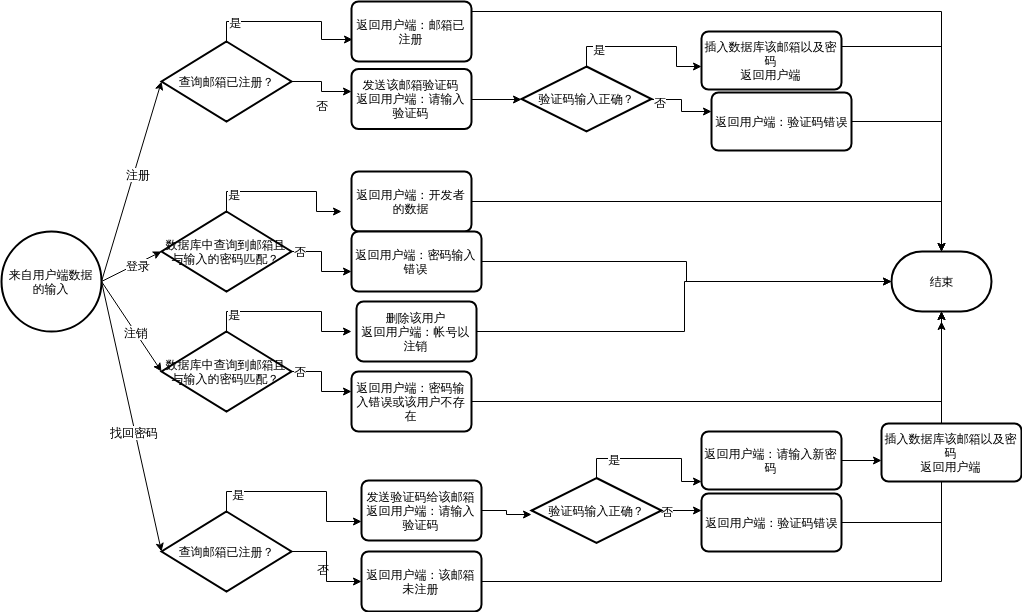
\includegraphics[width=14cm]{concrete_user_sys.png}
	\caption{用户管理系统事件时序} \label{fig:concrete_user_sys}
\end{figure}


数据流图\ref{fig:concrete_user_sys}明确表示了用户管理系统的运行


\textbf{C. 对异常情况的回应}

\begin{longtable}{|c|p{6cm}|p{6cm}|}
\caption{用户管理系统异常处理}\label{tab:developer_exception} \\
\hline
\textbf{异常类型} & \textbf{异常描述} & \textbf{异常处理}\\
\hline
\endfirsthead
%\multicolumn{3}{c}{\tablename\ \thetable\ -- \textit{Continued from previous page}} \\
\hline
\textbf{异常类型} & \textbf{异常描述} & \textbf{异常处理}\\
\hline
\endhead
\hline 
%\multicolumn{3}{r}{\textit{Continued on next page}} \\
\endfoot
\hline
\endlastfoot
通信失败 & 
与用户端采用网络通信,限定时间内没有收到应答或者没有新的请求 &
储存错误状态,断开连接\\
数据库异常 & 数据库出现异常,比如数据库断联,数据库储存满 &
暂停服务,通知管理员\\
攻击检测 & 网络安全相关,比如检测到某个账户持续性注册注销 &
停止对该帐号的应答,并且设定恢复时间\\
\end{longtable}

表\ref{tab:developer_exception}概要性描述了几个可能出现的错误,以及相关的解决方案。
更加详细的方案见概要设计。



\textbf{D. 用于把系统输入转换到相应输出的任何方法}

用户系统的处理主要是对数据库的访问处理,根据数据流图\ref{fig:concrete_user_sys}的
业务逻辑处理即可,并不需要额外的方程式或者数学算法。
		
\textbf{E. 对输出数据的有效性检测}

输出内容分为两类,一是返回给用户端的提示与错误信息:主体为文本内容,并且为每个信息配有unsigned int类型的描述符。
相关信息有:邮箱已注册;邮箱未注册;输入验证码;密码错误;

\begin{longtable}{|p{7cm}|p{7cm}|}
\caption{用户管理系统输出有效性检测}\label{tab:concrete_user_sys_output_valid} \\
\hline
\textbf{输出内容} & \textbf{有效性检测} \\
\hline
\endfirsthead
%\multicolumn{2}{c}{\tablename\ \thetable\ -- \textit{Continued from previous page}} \\
\hline
\textbf{输出内容} & \textbf{有效性检测} \\
\hline
\endhead
\hline 
%\multicolumn{2}{r}{\textit{Continued on next page}} \\
\endfoot
\hline
\endlastfoot
用户名 & 不为空,默认为邮箱,可进行修改 \\
姓名 & 不为空,中文或英文字符串,Unicode格式,限制长度64bytes \\
性别 & 可为空,男/女 \\
年龄 & 可为空,类型为unsigned int \\
下载/购买的应用ID & 可为空,类型为unsigned int, 全局唯一code \\
\end{longtable}


另外就是返回用户的信息,
见表\ref{tab:concrete_user_sys_output_valid}

\subsubsection{输出}

需求编码为SRS\_Server\_App\_P01\_O01

\begin{longtable}{|p{3cm}|p{4cm}|p{1cm}|p{6cm}|}
\caption{用户管理系统输出}\label{tab:concrete_user_sys_output} \\
\hline
\textbf{输出内容} & \textbf{输出位置} & \textbf{数量}  & \textbf{非法值处理错误信息}    \\
\hline
\endfirsthead
%\multicolumn{4}{c}{\tablename\ \thetable\ -- \textit{Continued from previous page}} \\
\hline
\textbf{输出内容} & \textbf{输出位置} & \textbf{数量}  & \textbf{非法值处理错误信息}  \\
\hline
\endhead
\hline 
%\multicolumn{4}{r}{\textit{Continued on next page}} \\
\endfoot
\hline
\endlastfoot
用户名 & 用户端 & 1 & 用户名不存在\\
姓名 & 用户端 & 1 & 姓名字符含有非法字符\\
性别 & 用户端 & 0/1 & 无\\
年龄 & 用户端 & 0/1 & 无\\
下载/购买的应用ID & 用户端 & $\ge 0$ & 无\\
注册的用户名密码 & 数据库 & 1 & 该用户已注册\\
注销的用户名密码 & 数据库 & 1 & 该用户未注册 \\
\end{longtable}
	
对输出数据的管理见表\ref{tab:concrete_user_sys_output}

\subsection{服务器端.第三方管理系统}

需求编码为SRS\_Server\_Other\_P01
\subsubsection{介绍}
第三方用户主要是广告投放、监督、资助,用户权限很大而且用户很少,不应当对外提供接口,
而应当交由管理员处理。

需求编码为SRS\_Server\_Other\_P01\_F01

\subsubsection{输入}

需求编码为SRS\_Server\_Other\_P01\_I01

\begin{longtable}{|p{3cm}|p{4cm}|p{1cm}|p{6cm}|}
\caption{第三方管理系统输入}\label{tab:concrete_other_sys_input} \\
\hline
\textbf{输入内容} & \textbf{输入来源} & \textbf{数量}  & \textbf{有效范围}    \\
\hline
\endfirsthead
%\multicolumn{4}{c}{\tablename\ \thetable\ -- \textit{Continued from previous page}} \\
\hline
\textbf{输入内容} & \textbf{输入来源} & \textbf{数量}  & \textbf{有效范围}  \\
\hline
\endhead
\hline 
%\multicolumn{4}{r}{\textit{Continued on next page}} \\
\endfoot
\hline
\endlastfoot
广告 & 广告投放机构 & $\ge 0$ & 符合法律的广告内容 \\
资助 & 公益单位或个人或广告投放机构 & $\ge 0$ & 符合转账条款 \\
监督 & 官方或公司 & &\\
\end{longtable}
对输入的管理信息见表\ref{tab:concrete_other_sys_input}	

\subsubsection{处理}
包含对输入数据所执行的所有操作和如何获得输出的过程

需求编码为SRS\_Server\_Other\_P01\_H01

\textbf{A. 输入数据的有效性检测}

交由管理员处理,此处不需要

\textbf{B. 操作的确切次序,包括各事件的时序}

交由管理员处理,此处不需要

\textbf{C. 对异常情况的回应}

交由管理员处理,此处不需要

\textbf{D. 用于把系统输入转换到相应输出的任何方法}

		
\textbf{E.	对输出数据的有效性检测}

交由管理员处理,此处不需要

\subsubsection{输出}

需求编码为SRS\_Server\_Other\_P01\_O01

交由管理员处理,此处不需要

{\color{red}

\subsection{服务器端.应用开发管理系统}

需求编码为SRS\_Server\_DevSys\_P01
\subsubsection{介绍}
集中处理开发者端的开发界面和用户端的个性化界面的数据计算,包括编译执行、debug.

处理完的数据需要传输给开发者端或者用户端显示给客户。

需求编码为SRS\_Server\_DevSys\_P01\_F01
\subsubsection{输入}

需求编码为SRS\_Server\_DevSys\_P01\_I01

本支系统针对开发者端和用户端,数据来源都是相应的开发或个性化界面。

输入数据要求

\begin{longtable}[]{@{}ll@{}}
\toprule
数据名称 & 数据要求\tabularnewline
\midrule
\endhead
命令 & 经过语法检查的指令,拥有执行权限,并且可执行\tabularnewline
代码 &
经过语法检查的字符串\tabularnewline
配置 & 由相应应用提供的对外配置接口 \tabularnewline
\bottomrule
\end{longtable}


\subsubsection{处理}

对输入进行处理,得到输出内容

需求编码为SRS\_Server\_DevSys\_P01\_H01

\textbf{A. 输入数据的有效性检测}

\begin{longtable}[]{@{}ll@{}}
\caption{应用开发管理系统输入的有效性检测}\label{tab:concrete_DevSyS_input_valid}\\
\toprule
数据名称 & 数据要求\tabularnewline
\midrule
\endhead
命令 & 拥有执行权限,并且可执行\tabularnewline
代码 & 不含攻击特征 \tabularnewline
配置 & 符合接口特征且不含攻击特征 \tabularnewline
\bottomrule
\end{longtable}

见表\ref{tab:concrete_DevSyS_input_valid}

\textbf{B. 操作的确切次序,包括各事件的时序}

分成两类事件,来自开发者端的应用开发界面或者来自客户端的应用个性化界面。

处理的流程类似,均为按照代码进行编译执行,返回信息以及执行数据。


\textbf{C. 对异常情况的回应}

\begin{longtable}{|c|p{6cm}|p{6cm}|}
\caption{用户管理系统异常处理}\label{tab:server_DevSys_exception} \\
\hline
\textbf{异常类型} & \textbf{异常描述} & \textbf{异常处理}\\
\hline
\endfirsthead
%\multicolumn{3}{c}{\tablename\ \thetable\ -- \textit{Continued from previous page}} \\
\hline
\textbf{异常类型} & \textbf{异常描述} & \textbf{异常处理}\\
\hline
\endhead
\hline 
%\multicolumn{3}{r}{\textit{Continued on next page}} \\
\endfoot
\hline
\endlastfoot
通信失败 & 
与用户端采用网络通信,限定时间内没有收到应答或者没有新的请求 &
储存错误状态,断开连接\\
数据库异常 & 数据库出现异常,比如数据库断联,数据库储存满 &
暂停服务,通知管理员\\
攻击检测 & 网络安全相关,比如检测到某个账户持续性注册注销 &
停止对该帐号的应答,并且设定恢复时间\\
编译失败 & 代码或者配置错误 & 立即停止,并且返回相应终端错误信息 \\
执行失败 & 出现诸如0除或者内存爆炸的执行错误 & 立即停止,并且返回相应终端错误信息\\
\end{longtable}

表\ref{tab:server_DevSys_exception}概要性描述了几个可能出现的错误,以及相关的解决方案。
更加详细的方案见概要设计。



\textbf{D. 用于把系统输入转换到相应输出的任何方法}

编译执行
		
\textbf{E. 对输出数据的有效性检测}

输出为编译运行的信息或者界面数据,无需过多有效性检测

\subsubsection{输出}

需求编码为SRS\_Server\_DevSys\_P01\_O01

输出为编译运行的信息或者界面数据
}

\subsection{客户端.应用管理}
本小节主要描述了普通用户进行应用管理的需求,包括应用查询、购买、安装、删除等等。

需求编码为SRS\_User\_App\_P01
\subsubsection{介绍}
逐条列出与本特性相关的功能需求。包括项目如何响应预期的错误输入,非法条件和无效输入。需求应该简明,完整,不含糊,可验证,必要的。 当需要的信息不确定的时候使用“待定”。
需求编码为SRS\_User\_App\_P01\_F01

\subsubsection{输入}

需求编码为SRS\_User\_App\_P01\_I01

针对普通客户对应用的查询管理需求,数据来源均为客户(此处不考虑隐式的数据来源,即服务器),具体如下:

\begin{longtable}[]{@{}ll@{}}
\toprule
数据名称 & 数据要求\tabularnewline
\midrule
\endhead
应用id & 无要求(应用查询),应用必须存在于应用商店中(应用购买、应用更新、应             用安装),应用必须存在于本地(删除)\tabularnewline
对应用的操作 & 查询、购买、安装、更新、删除之一\tabularnewline
银行账号 & 当且仅当购买应用时不为空,为合法的银行账号\tabularnewline
\bottomrule
\end{longtable}

\subsubsection{处理}
对输入进行处理,得到输出内容

需求编码为SRS\_User\_App\_P01\_H01

\textbf{A. 输入数据的有效性检测}

\begin{longtable}[]{@{}ll@{}}
\caption{客户端进行应用管理输入数据的有效性检测}\label{tab:client_app_management}\\
\toprule
数据名称 & 数据要求\tabularnewline
\midrule
\endhead
应用id & 无要求(应用查询),应用必须存在于应用商店中(应用购买、应用更新、应             用安装),应用必须存在于本地(删除)\tabularnewline
对应用的操作 & 查询、购买、安装、更新、删除之一\tabularnewline
银行账号 & 当且仅当购买应用时不为空,为合法的银行账号\tabularnewline
\bottomrule
\end{longtable}

见表\ref{tab:client_app_management}

\textbf{B. 操作的确切次序,包括各事件的时序}

\begin{figure}[ht]
	\centering
	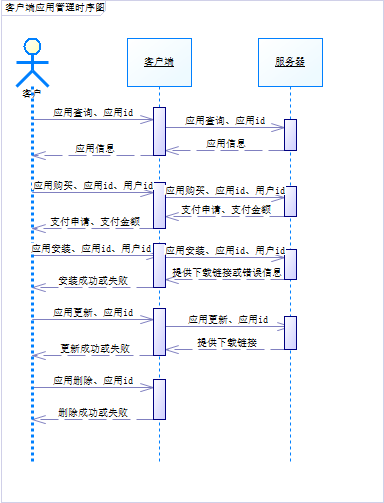
\includegraphics[width=14cm]{client_app_order.png}
	\caption{客户端进行应用管理的事件时序} \label{fig:client_app_order}
\end{figure}
见图\ref{fig:client_app_order}

\textbf{C. 对异常情况的回应}

\begin{longtable}{|c|p{6cm}|p{6cm}|}
\caption{客户端应用管理异常处理}\label{tab:client_app_management_exception}\\
\hline
\textbf{异常类型} & \textbf{异常描述} & \textbf{异常处理}\\
\hline
\endfirsthead

\hline
\textbf{异常类型} & \textbf{异常描述} & \textbf{异常处理}\\
\hline
\endhead
\hline 
\endfoot
\hline
\endlastfoot
服务器异常 & 
与服务器采用网络通信,限定时间内没有收到应答 &
储存错误状态,提示用户检查网络连接\\
应用id不合法 
& id对应的应用并不存在于本地(更新、删除),id对应的应用并不存在于应用商店(购买、安装、更新)
& 提示用户重新操作\\
本地磁盘空间不足
& 本地磁盘空间不足导致应用无法安装
& 提示用户释放本地磁盘空间\\
\end{longtable}

表\ref{tab:client_app_management_exception}概要性描述了几个可能出现的错误,以及相关的解决方案。
更加详细的方案见概要设计。

\textbf{D. 用于把系统输入转换到相应输出的任何方法}
只需要将服务器返回的结果返回给用户即可,不需要额外的数学算法或操作逻辑等等。
		
\textbf{E. 对输出数据的有效性检测}

此处只考虑客户端返回给客户的数据,返回给服务器的数据参见服务器端.用户管理系统。
输出数据为:操作的成功与否以及可能的错误信息,具体如下:
\begin{longtable}{|p{7cm}|p{7cm}|}
\caption{开发者端应用管理输出有效性检测}\label{tab:concrete_dev_sys_output_valid} \\
\hline
\textbf{输出内容} & \textbf{有效性检测} \\
\hline
\endfirsthead
\hline
\textbf{输出内容} & \textbf{有效性检测} \\
\hline
\endhead
\hline 
\endfoot
\hline
\endlastfoot

操作结果 & 布尔量,成功或失败 \\
查询结果 & 若干个元组,每个元组表示相关的应用的信息,可以为空\\
错误信息 & 操作成功则为空,操作失败则为一个字符串,建议开发者下一步的操作,长度暂定为128byte,具体参见对异常情况的回应部分\\
\end{longtable}


\subsubsection{输出}

需求编码为SRS\_User\_App\_P01\_O1

参见上一节E对输出数据的有效性检测。



\subsection{客户端.信息反馈}
本小节主要描述了普通用户进行信息反馈的需求,包括应用评分、评价等等。

需求编码为SRS\_User\_Info\_P01
\subsubsection{介绍}
逐条列出与本特性相关的功能需求。包括项目如何响应预期的错误输入,非法条件和无效输入。需求应该简明,完整,不含糊,可验证,必要的。 当需要的信息不确定的时候使用“待定”。

需求编码为SRS\_User\_Info\_P01\_F01

\subsubsection{输入}

针对客户对应用进行评价的需求,输入数据应当包括:应用id、评价、评分等等,数据来源均为客户,具体如下:

需求编码为SRS\_User\_Info\_P01\_I01

\begin{longtable}[]{@{}ll@{}}
\toprule
数据名称 & 数据要求\tabularnewline
\midrule
\endhead
应用id & 应用id为该客户本地已安装的应用之一\tabularnewline
评分 & 1-5之间的整型数字,可以为空\tabularnewline
评论 & 一个字符串,长度暂定为256字节,可以为空\tabularnewline
\bottomrule
\end{longtable}

\subsubsection{处理}
对输入进行处理,得到输出内容

需求编码为SRS\_User\_Info\_P01\_H01

\textbf{A. 输入数据的有效性检测}

\begin{longtable}[]{@{}ll@{}}
\caption{客户端信息反馈的输入数据的有效性检测}\label{tab:client_app_info}\\
\toprule
数据名称 & 数据要求\tabularnewline
\midrule
\endhead
具体需求 & 应用信息查询、评论回复、收入查询、收入提现、收入转账等命令之一\tabularnewline
应用id & 当且仅当具体需求是应用信息查询时不为空,应用id为该开发者开发的应用之一\tabularnewline
评论回复 & 当且仅当具体需求是评论回复时不为空,为一个字符串,长度暂定为256字节\tabularnewline
银行账号 & 当且仅当具体需求是收入提现或转账时不为空,为一个合法的银行账号\tabularnewline
\bottomrule
\end{longtable}

见表\ref{tab:client_app_info}

\textbf{B. 操作的确切次序,包括各事件的时序}

\begin{figure}[ht]
	\centering
	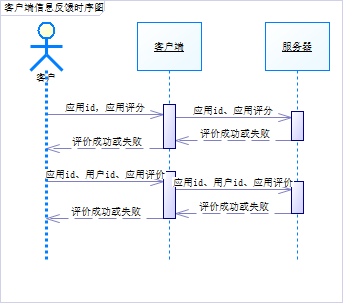
\includegraphics[width=14cm]{client_info_order.png}
	\caption{开发者获取信息反馈并处理的事件时序} \label{fig:client_info_order}
\end{figure}
见图\ref{fig:client_info_order}

\textbf{C. 对异常情况的回应}

\begin{longtable}{|c|p{6cm}|p{6cm}|}
\caption{开发者端信息反馈异常处理}\label{tab:client_info_exception}\\
\hline
\textbf{异常类型} & \textbf{异常描述} & \textbf{异常处理}\\
\hline
\endfirsthead

\hline
\textbf{异常类型} & \textbf{异常描述} & \textbf{异常处理}\\
\hline
\endhead
\hline 
\endfoot
\hline
\endlastfoot
服务器异常 & 
与服务器采用网络通信,限定时间内没有收到应答 &
储存错误状态,提示开发者检查网络连接\\
应用id不合法 
& id对应的应用并未在用户本地安装
& 提示开发者重新操作
\end{longtable}

表\ref{tab:client_info_exception}概要性描述了几个可能出现的错误,以及相关的解决方案。
更加详细的方案见概要设计。

\textbf{D. 用于把系统输入转换到相应输出的任何方法}
只需要将服务器返回的结果返回给用户即可,不需要额外的数学算法或操作逻辑等等。
		
\textbf{E. 对输出数据的有效性检测}

此处只考虑客户端返回给客户的数据,返回给服务器的数据参见服务器端.客户管理系统。具体如下:
\begin{longtable}{|p{7cm}|p{7cm}|}
\caption{客户端信息反馈输出有效性检测}\label{tab:concrete_dev_sys_output_valid} \\
\hline
\textbf{输出内容} & \textbf{有效性检测} \\
\hline
\endfirsthead
\hline
\textbf{输出内容} & \textbf{有效性检测} \\
\hline
\endhead
\hline 
\endfoot
\hline
\endlastfoot
操作结果 & 布尔量

\end{longtable}


\subsubsection{输出}
需求编码为SRS\_User\_Info\_P01\_O01

参见上一节E对输出数据的有效性检测。



{\color{red}

\subsection{客户端.应用个性化界面}

本小节主要描述了普通用户对应用进行配置并运行预览的界面。

需求编码为SRS\_User\_Dev\_P01
\subsubsection{介绍}

不同的用户对同一个应用可能有不同的需求,使用配置接口,设定不同的从参数,获得不同的
应用版本。

需求编码为SRS\_User\_Dev\_P01\_F01

\subsubsection{输入}

用户的输入主要是配置的参数,依据不同应用给出的接口而定。

同时应用的开发人员也需要明确指出不同的参数配置方式。并且与接口相接。

需求编码为SRS\_User\_Dev\_P01\_I01


\subsubsection{处理}
对输入进行处理,得到输出内容

需求编码为SRS\_User\_Dev\_P01\_H01

\textbf{A. 输入数据的有效性检测}

符合配置接口定义即可,无需其他有效性检测。

\textbf{B. 操作的确切次序,包括各事件的时序}

配置好的参数返回服务器,进行运行预览。

预览的结果返回本界面。

\textbf{C. 对异常情况的回应}

\begin{longtable}{|c|p{6cm}|p{6cm}|}
\caption{开发者端信息反馈异常处理}\label{tab:client_info_exception}\\
\hline
\textbf{异常类型} & \textbf{异常描述} & \textbf{异常处理}\\
\hline
\endfirsthead

\hline
\textbf{异常类型} & \textbf{异常描述} & \textbf{异常处理}\\
\hline
\endhead
\hline 
\endfoot
\hline
\endlastfoot
服务器异常 & 
与服务器采用网络通信,限定时间内没有收到应答 &
储存错误状态,提示开发者检查网络连接\\
应用id不合法 
& id对应的应用并未在用户本地安装
& 提示开发者重新操作
\end{longtable}

表\ref{tab:client_info_exception}概要性描述了几个可能出现的错误,以及相关的解决方案。
更加详细的方案见概要设计。

\textbf{D. 用于把系统输入转换到相应输出的任何方法}
只需要将服务器返回的结果返回给用户即可,不需要额外的数学算法或操作逻辑等等。
		
\textbf{E. 对输出数据的有效性检测}

此处只考虑客户端返回给客户的数据,返回给服务器的数据参见服务器端.客户管理系统。具体如下:
\begin{longtable}{|p{7cm}|p{7cm}|}
\caption{客户端信息反馈输出有效性检测}\label{tab:concrete_dev_sys_output_valid} \\
\hline
\textbf{输出内容} & \textbf{有效性检测} \\
\hline
\endfirsthead
\hline
\textbf{输出内容} & \textbf{有效性检测} \\
\hline
\endhead
\hline 
\endfoot
\hline
\endlastfoot
操作结果 & 布尔量

\end{longtable}


\subsubsection{输出}
需求编码为SRS\_User\_Dev\_P01\_O01

参见上一节E对输出数据的有效性检测。

}

\section{性能需求}

\subsection{开发者端性能}
需求编码为SRS\_NF\_P1\_E01

开发者端的性能主要依赖于服务器的性能,例如:上传、更新、删除应用的请求应当在1秒内得到相应,可以向服务器并行提交并执行多个请求。

\subsection{客户端性能}
需求编码为SRS\_NF\_P1\_E02

客户端的性能也主要依赖于服务器的性能,例如:对应用的查询、购买、安装等操作应当在1秒内得到相应。
但客户端还需要独自管理本地已安装的应用,这里要求客户端能够在1秒内列出本地所有通过应用商店安装的应用。

\subsection{服务器性能}
需求编码为SRS\_NF\_P1\_E03

本子章节应从整体上描述静态和动态的量化的对软件(或人与软件交互)的需求。

\begin{longtable}{|p{4cm}|p{10cm}|}
\caption{服务器性能}\label{tab:concrete_performance_server} \\
\hline
\textbf{性能需求} & \textbf{需求的具体内容}     \\
\hline
\endfirsthead
%\multicolumn{4}{c}{\tablename\ \thetable\ -- \textit{Continued from previous page}} \\
\hline
\textbf{性能需求} & \textbf{需求的具体内容}    \\
\hline
\endhead
\hline 
%\multicolumn{4}{r}{\textit{Continued on next page}} \\
\endfoot
\hline
\endlastfoot
支持的开发者数 & 100,000 \\
支持的用户数 & 1,000,000 \\
并发开发者数 & 1,000 \\
并发用户数 & 100,000 \\
应用大小限制 & 100G(更大的需要申请)\\
应用总数 & 100,000,000 \\
\end{longtable}

服务器的性能需求见表\ref{tab:concrete_performance_server}

\section{外部接口需求}
\subsection{用户接口}
需求编码为SRS\_UserInter\_01

\begin{longtable}{|p{4cm}|p{7cm}|p{7cm}|}
	\caption{开发者与应用商店系统的接口}\label{tab:developer_interface} \\
	\hline
	\textbf{开发者需求} & \textbf{输入} & \textbf{输出}\\
	\hline
	\endfirsthead
	\hline
	\textbf{开发者需求} & \textbf{输入} & \textbf{输出}\\
	\hline
	\endhead
	\hline 
	\endfoot
	\hline
	\endlastfoot
	登录 & 账号、密码 & 登录成功与否\\
	注册 & 账号、密码 & 注册成功与否\\
	应用上传 & 本地应用 & 上传成功与否\\
	应用更新 & 本地应用和待更新应用id & 更新成功与否\\
	应用删除 & 待删除应用id & 删除成功与否\\
	收入查询 & 无 & 收入\\
	评论回复 & 回复内容 & 回复成功与否\\
	\end{longtable}

\begin{longtable}{|p{4cm}|p{7cm}|p{7cm}|}
	\caption{普通用户与应用商店系统的接口}\label{tab:client_interface} \\
	\hline
	\textbf{用户需求} & \textbf{输入} & \textbf{输出}\\
	\hline
	\endfirsthead
	\hline
	\textbf{用户需求} & \textbf{输入} & \textbf{输出}\\
	\hline
	\endhead
	\hline 
	\endfoot
	\hline
	\endlastfoot
	登录 & 账号、密码 & 登录成功与否\\
	注册 & 账号、密码 & 注册成功与否\\
	应用查询 & 应用id & 相关的应用,以列表呈现\\
	应用购买 & 待购买应用id和银行账户 & 购买成功与否\\
	应用安装 & 待安装应用id & 安装成功与否\\
    应用删除 & 待删除应用id & 删除成功与否\\
	应用评分 & 待评价应用id和评分 & 评分成功与否\\
	应用评价 & 待评价应用id和评论 & 评论成功与否\\
	\end{longtable}
开发者和普通用户与该应用商店系统之间的接口分别参见表\ref{tab:developer_interface}和表\ref{tab:client_interface}。

输入、输出的时序关系参见之前的功能需求部分。

另外,应用商店系统的还包含help选项和一定的异常处理,提示开发者和普通用户如何正确操作。

\subsection{软件接口}

需求编码为SRS\_SoftInter\_01

该应用商店系统与外部有关联的软件只有操作系统和数据库。
\begin{longtable}{|p{4cm}|p{10cm}|}
\caption{操作系统与应用商店系统的接口}\label{tab:os_interface} \\
\hline
\textbf{接口目的} & \textbf{接口形式}\\
\hline
\endfirsthead
\hline
\textbf{接口目的} & \textbf{接口形式}\\
\hline
\endhead
\hline 
\endfoot
\hline
\endlastfoot
在本地安装应用 & bool install(package,loaction),package为软件包的文件描述符,location为安装目录\\
删除本地应用 & bool uninstall(uninstallProgram),uninstallProgram为卸载程序的文件描述符\\
\end{longtable}

\begin{longtable}{|p{4cm}|p{10cm}|}
	\caption{数据库与应用商店系统的接口}\label{tab:db_interface} \\
	\hline
	\textbf{接口目的} & \textbf{接口形式}\\
	\hline
	\endfirsthead
	\hline
	\textbf{接口目的} & \textbf{接口形式}\\
	\hline
	\endhead
	\hline 
	\endfoot
	\hline
	\endlastfoot
	查询应用信息 & app searchApp(id),id为应用id,app为一个结构体,包含了有关该应用的信息\\
	查询用户信息 & client searchClient(account),account为用户账号,client为一个结构体,包含了有关该用户的信息\\
	查询开发者信息 & developer searchDeveloper(account),account为开发者账号,developer为一个结构体,包含了有关该开发者的信息\\
	修改应用信息 & bool updateApp(app),app为一个结构体,也可用此接口新增应用\\
	修改用户信息 & bool updateClient(client),client为一个结构体,也可用此接口新增用户\\
	修改开发者信息 & bool updateDeveloper(developer),developer为一个结构体,也可用此接口新增开发者\\
	\end{longtable}
该应用商店系统和操作系统及数据库的接口分别参见表\ref{tab:os_interface}和表\ref{tab:db_interface}。

\subsection{硬件接口}

需求编码为SRS\_HardInter\_01

该应用商店系统不需要使用外部的硬件设备如打印机等等,故无需考虑硬件接口。

\subsection{通讯接口}

需求编码为SRS\_CommInter\_01

服务器端、客户端和开发者端之间的通信均采用TCP/IP协议。